\chapter{Clustering}

Nous avons expérimentés plusieurs méthodes de clustering pour extraire des points d'intêrets à partir des données
des quelques 80 000 photos que nous possédons.

Nous présentons dans cette partie les méthodes que nous avons utilisées, leur pertinence dans le cadre de ce projet, et
autres avantages et/ou inconvénients.

Nous avons principalement fais un clustering basé sur la latitude/longitude. Nous montrons néanmoins (dans la partie K-Means) qu'un clustering sur d'autres critères, par exemple le mois de prise de la photo, ne donne pas de résultats satisfaisant.

\section{Clustering hiérarchique}
    Cette méthode, bien qu'utile quand on ne connaît pas le nombre de clusters
    attendu (comme c'est le cas dans ce projet), ne passe pas à l'échelle~:
    son exécution sur la totalité du jeu de donnée provoque un dépassement de mémoire.

    Nous avons malgré tout réalisé un échantillonnage aléatoire (de 1,000 lignes)
    de notre jeu de données sur lequel on a effectué un \textit{clustering hiérarchique}
    afin d'avoir une idée sur le nombre de clusters qui pouvaient être extraits.

    \begin{figure}[H]
        \centering
        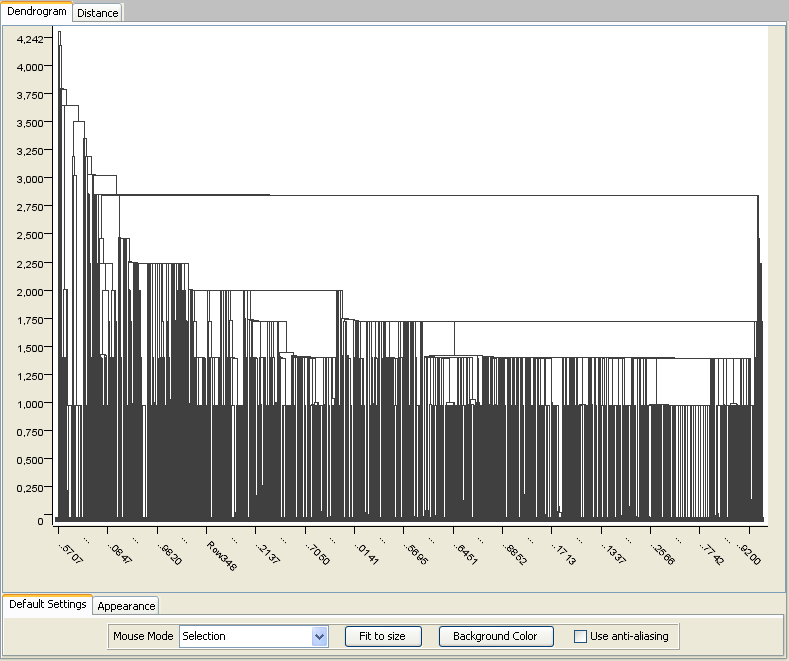
\includegraphics[scale=0.3]{../screenshots/hierarchical_clustering_1000_samples.png}
        \caption{Résultat du clusturing hiérarchique sur 1000 échantillons}
        \label{diagram:hierarchical_clustering_1000_samples}
    \end{figure}

    Mais même sur un jeu de données aussi restreint (par rapport aux données
    originales), le résultat était difficilement exploitable (car très dense),
    et le fait que les données exploitées représentaient moins de $5\%$ des
    données originales faisait que ce clustering était fort instable (structure
    variant sur des samplings différents).

\section{K-Means}
    Bien que plus rapide à l'execution que le clustering hiérarchique (et moins demandant en ressources mémoire),
    le clustering K-Means n'est pas des plus adaptés pour ce projet~: il demande de connaitre le nombre de clusters et
    donne des clusters parfois répartis sur de grandes zones et moins denses que ce que donnent d'autres méthodes (notamment Mean Shift).

    \begin{figure}[H]
        \centering
        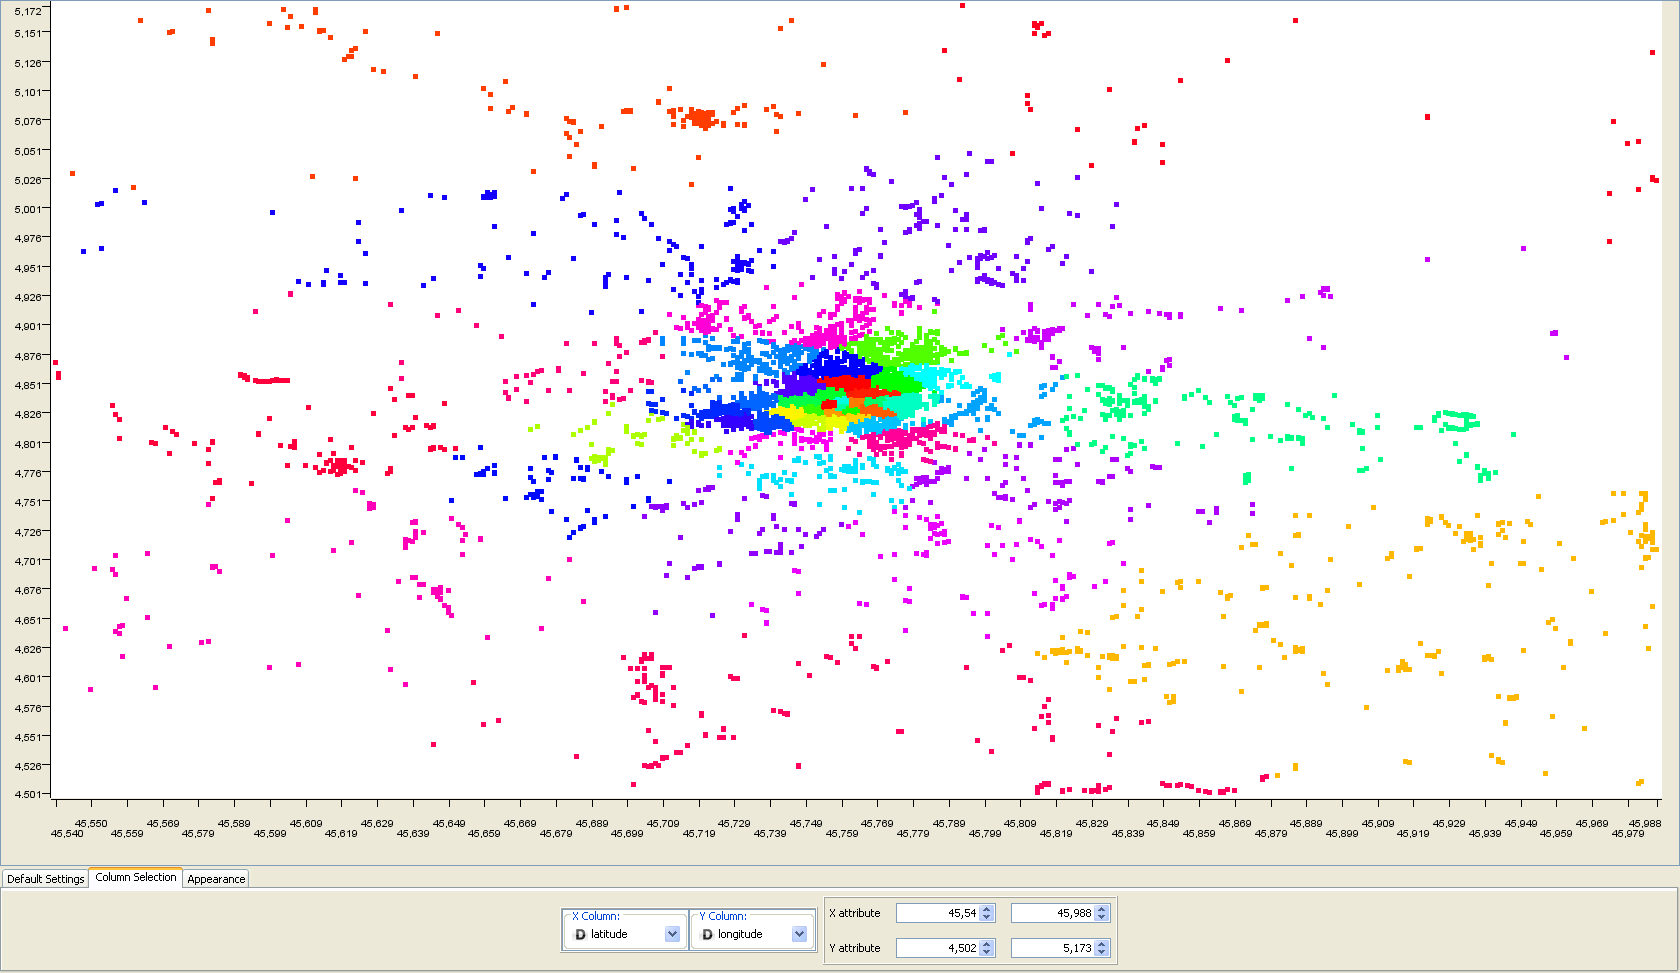
\includegraphics[scale=0.25]{../screenshots/kmeans_geographic.png}
        \caption{Résultat du clustering K-Means}
        \label{diagram:kmeans_geographic}
    \end{figure}

    Nous avons aussi essayé de réaliser des clusters en nous basant sur le mois de prise des photos, afin de montrer certaines tendances (quartier plus fréquentés pendant l'été, par exemple) mais les résultats étaient peu satisfaisants (pas de correlation particulière entre le mois de prise de la photo et sa position).

    \begin{figure}[H]
        \centering
        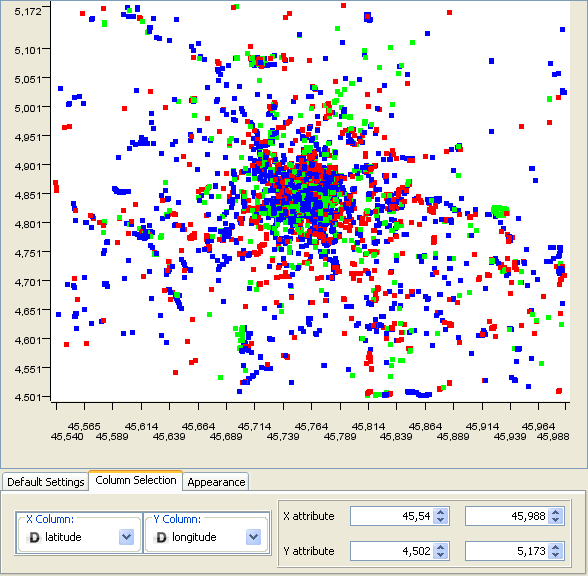
\includegraphics[scale=0.28]{../screenshots/kmeans_month.png}
        \caption{Résultat du clustering K-Means basé sur la date de prise des photos}
        \label{diagram:kmeans_month}
    \end{figure}


\section{DBScan}
    DBScan cumule les tares de K-Means et du clustering hiérarchique : très lent à s’exécuter (avec dépassement mémoire
    si on utilise la totalité du jeu de données) et donnant des clusters très dispersés, même bien moins denses que ceux de K-Means.


    \begin{figure}[H]
        \centering
        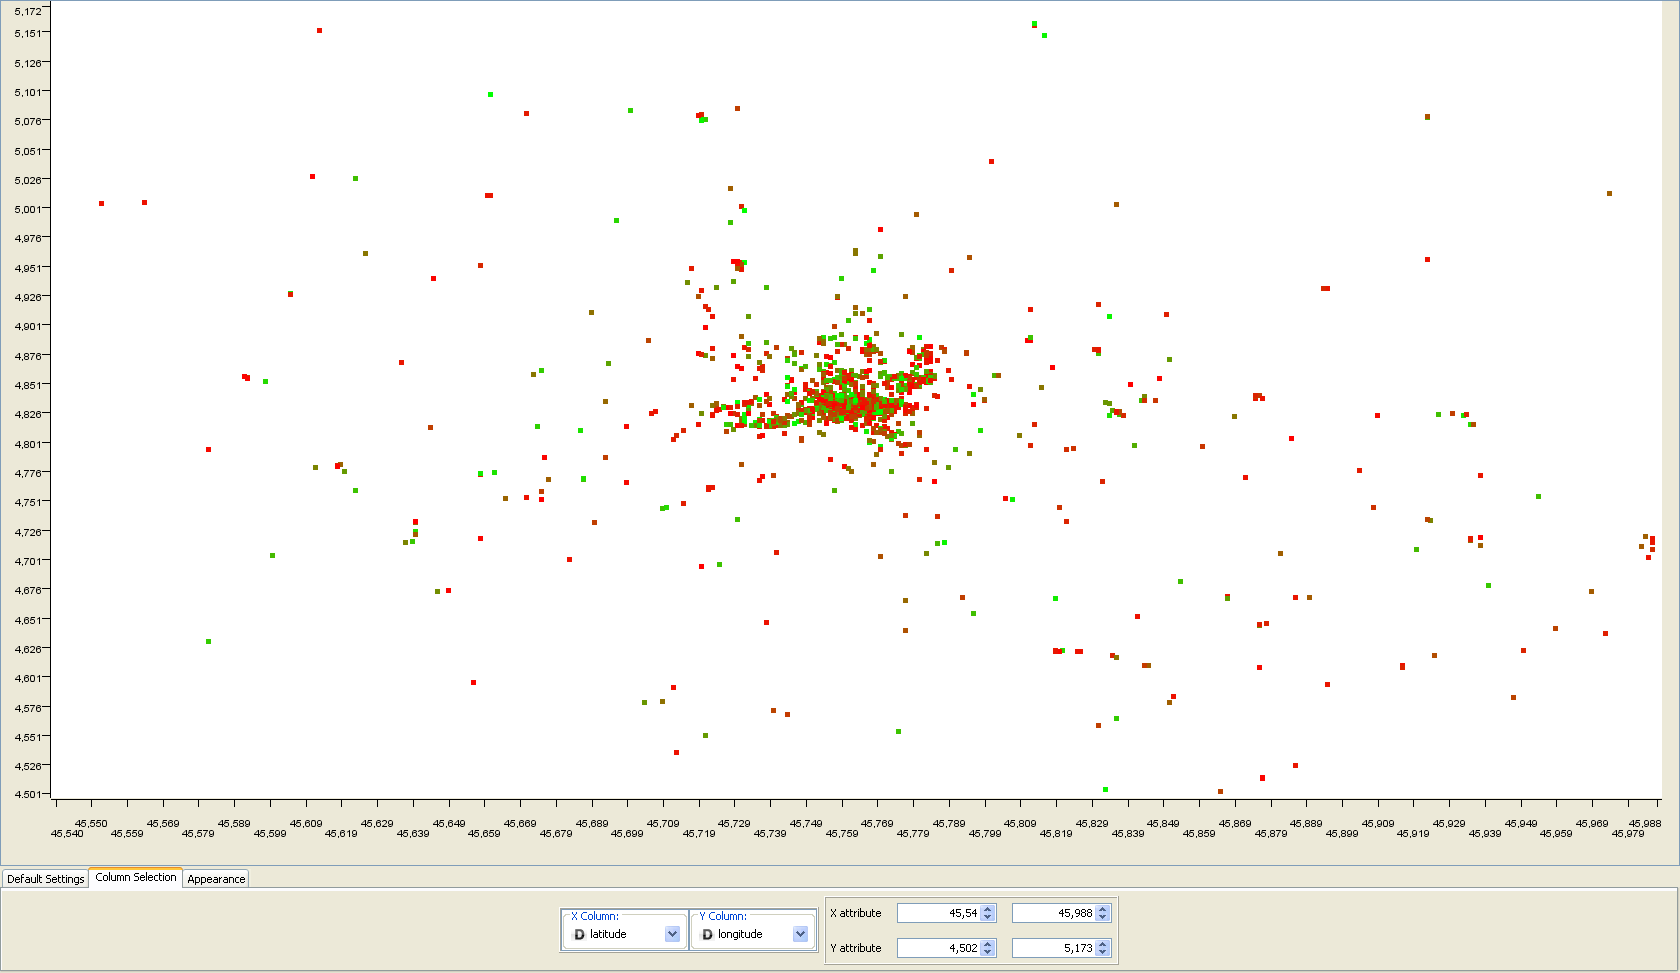
\includegraphics[scale=0.3]{../screenshots/dbscan_geographic.png}
        \caption{Résultat du clustering avec DBScan}
        \label{diagram:dbscan_geographic}
    \end{figure}


\section{Mean Shift}

    \textbf{TODO : finir cette partie}